\documentclass[12pt,a4paper]{report}
\setlength\textwidth{145mm}
 \setlength\topmargin{0mm}
 \setlength\headsep{0mm}
 \setlength\headheight{0mm}
 
% Přepneme na českou sazbu
\usepackage[czech]{babel}
\usepackage[IL2]{fontenc}
\usepackage{graphicx} 

%% Použité kódování znaků: obvykle latin2, cp1250 nebo utf8:
\usepackage[utf8]{inputenc}
\begin{document}


\section{Triviální versus Cache-oblivious implementace}
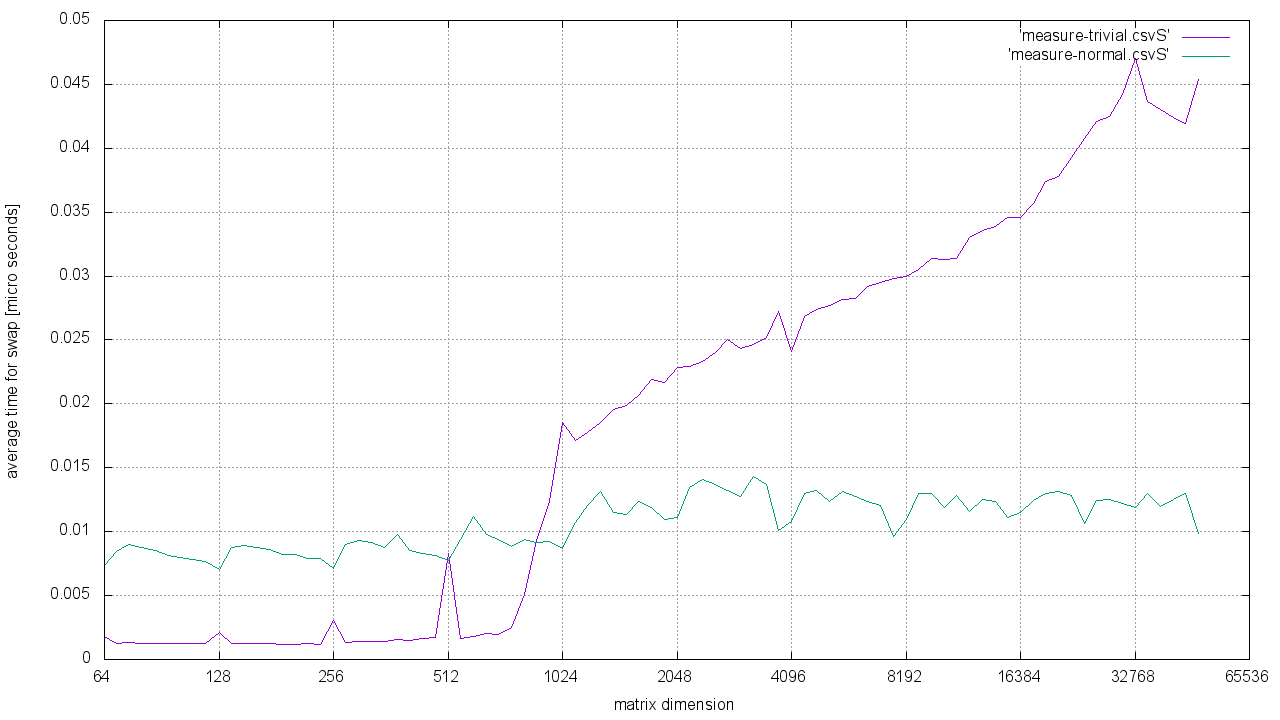
\includegraphics[width=\textwidth]{./tests/graph1.png}

Pro měření jsme dovolili použít až 10 GB paměti RAM.
Použitý počítač je osazen procesorem intel i7-920 @2.6 GHz
s 64-bitovými instrukecemi AMD64 a následujícími parametry cache:
\begin{itemize}
	\item L1 cache -- XXX,
	\item L2 cache -- XXX,
	\item L3 cache -- XXX,
\end{itemize}.

850 MB  -> N=15000
4,56 GB -> N=35000
7,54 GB -> N=45000




\section{Standartní vs naivní implementace}
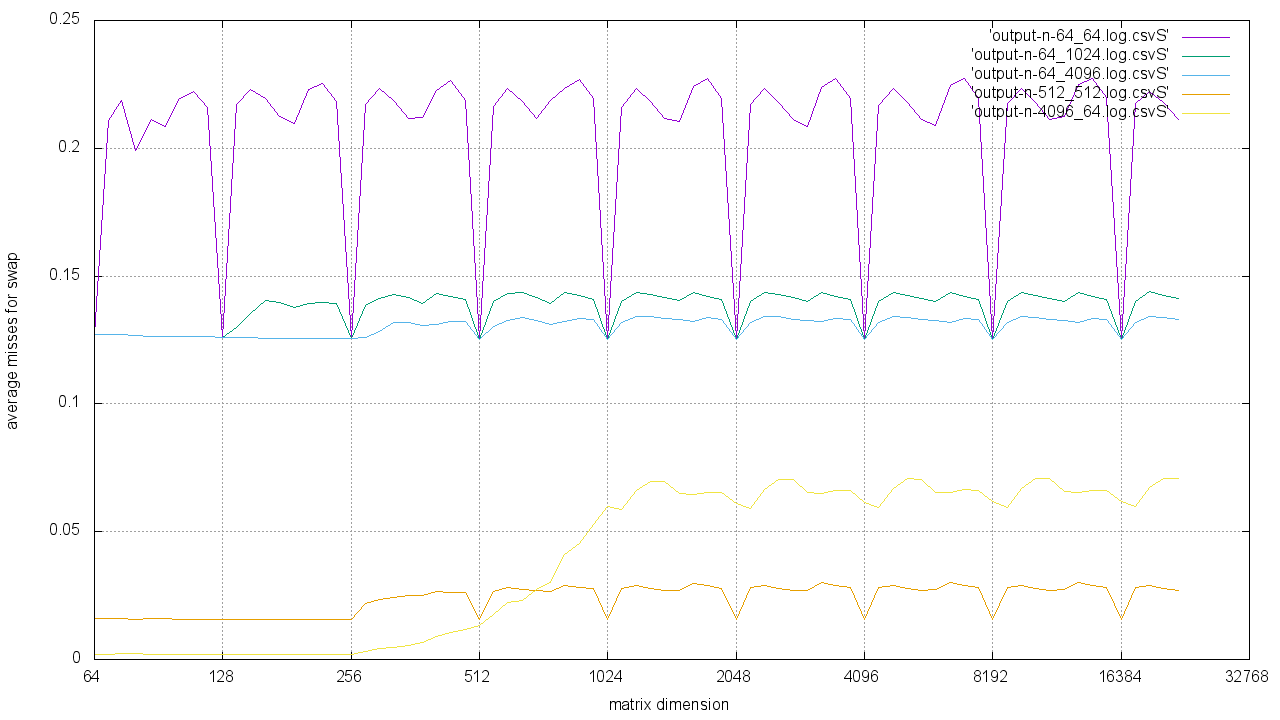
\includegraphics[width=\textwidth]{./tests/graph2.png}

Simulace jsme opět prováděly na stejných datech, jako při měření 
na počítači, nicměně pouze do maximalní velikosti matice 2 GB.
Předchozí graf znázorňuje závislost missů cache na počtu přístupů


  
\end{document}
